\section{Server}
\label{server}
Wie in Abschnitt \ref{app_architecture} beschrieben, müssen die aufgezeichneten Daten der Clientbibliothek weiter verarbeitet werden. % nochmal etwas genauer

Im Folgenden werden die zwei serverseitigen Komponenten, Datenbank und HTTP-Server, vorgestellt. 

%TODO: footnote ++ update

%TODO: subsection title ?!
\subsection{Virtuelle Maschine}

\subsubsection{Konfiguration}

Als Betriebssystem für den Server dient ein Debian in der Version 7.0. Der Maschine wurde 1 Prozessorkern und 512 MB RAM zugewiesen. Änderungen können im Vagrantfile, siehe Abschnitt \ref{vagrant}, oder der Virtual Box-Konfiguration vorgenommen werden.

Weitere Softwarequellen, welche installiert wurden, sind: 
\begin{description}
	\item[openSSH Server] 
	Dieser 
\end{description}


\subsubsection{Ordnerstruktur}
% TODO positioning, sizing
\begin{minipage}[c]{\textwidth} %Ordnerstruktur in Minipage damit die zusammengehalten wird
\dirtree{%
 .1 /serverside.
 .2 classes.
 .2 controllers.
 	.3 api.
 		.4 audio.js.
 		.4 captures.js.
 		.4 log.js.
 		.4 sessions.js.
 		.4 tasks.js.
 		.4 todos.js.
 		.4 videos.js.
 	.3 backend.js.
 	.3 frontend.js.
 .2 node\_modules.
 .2 public.
 	.3 css.
 		.4 plugins.
 		.4 bootstrap.min.css.
 		.4 bootstrap-theme.min.css.
 		.4 sb-admin.css.
 		.4 style.css.
 		.4 video-js.min.css.
 	.3 fonts.
 	.3 img.
 	.3 js.
 .2 uploads.
 .2 views.
}
\end{minipage}


\subsubsection{Vagrant}
\label{vagrant}
Um die Bereitstellung der Serverumgebung zu vereinfachen wurde die virtuelle Maschine mittels Vagrant\footnote{Vagrant: http://www.vagrantup.com/} konfiguriert. Vagrant ist ein Kommandozeilenwerkzeug um schnell reproduzierbare Entwicklungsumgebungen zu schaffen und diese später zu verteilen oder zu exportieren. Dabei wird Virtual Box als Virtualisierungssoftware eingesetzt. Aber auch VMware wird unterstützt. 

Die eigene VM wird mittels einer VM-Schablone (die eigentliche VM) und einer Konfigurationsdatei geladen, die alle Eigenschaften der VM bereithält, zum Beispiel Portweiterleitungen. Die Schablone kann demnach bereits einige Standardsoftwarepakete beinhalten. 

Auf dem Host-System können die gewohnten Entwicklungswerkzeuge eingesetzt werden, da der Ordner, indem Vagrant konfiguriert wurd, mit dem Ordner /Vagrant auf dem Gast-System synchronisiert wird. 

Auch die Entwicklung von Software mittels einer Vagrant VM ergibt einen gut zu bedienenden Arbeitsfluss. So ist es beispielsweise möglich mittels \textbf{vagrant up} und \textbf{vagrant ssh} die Maschine zu starten und darauf zu verbinden, ohne dabei extra overhead, wie zum Beispiel Fenster, zu erzeugen. Die SSH-Credentials folgen dem \textit{Convention over Configuration}-Paradigma. Username, sowie Passwort lauten standardmäßig vagrant. 


\subsection{Datenbank}

Zur persistenten Speicherung der Nutzdaten wird MySQL verwendet. MySQL bietet sich an, da es Verbreitung und Sicherheit bietet, sowie von Oracle als kommerzielles, wie auch Open Source-Derivat entwickelt wird. Das Projekt nutzt die Community-Server-Edition. 
%TODO: Links in footnotes

\subsubsection{Datenbank-Modell}
Das Datenbankmodell wurde mit Hilfe des MySQL Workbench erstellt. Die Abbildung \ref{figure-db-model} zeigt das Ergebnis.
\begin{figure}[h!]
	\centering
	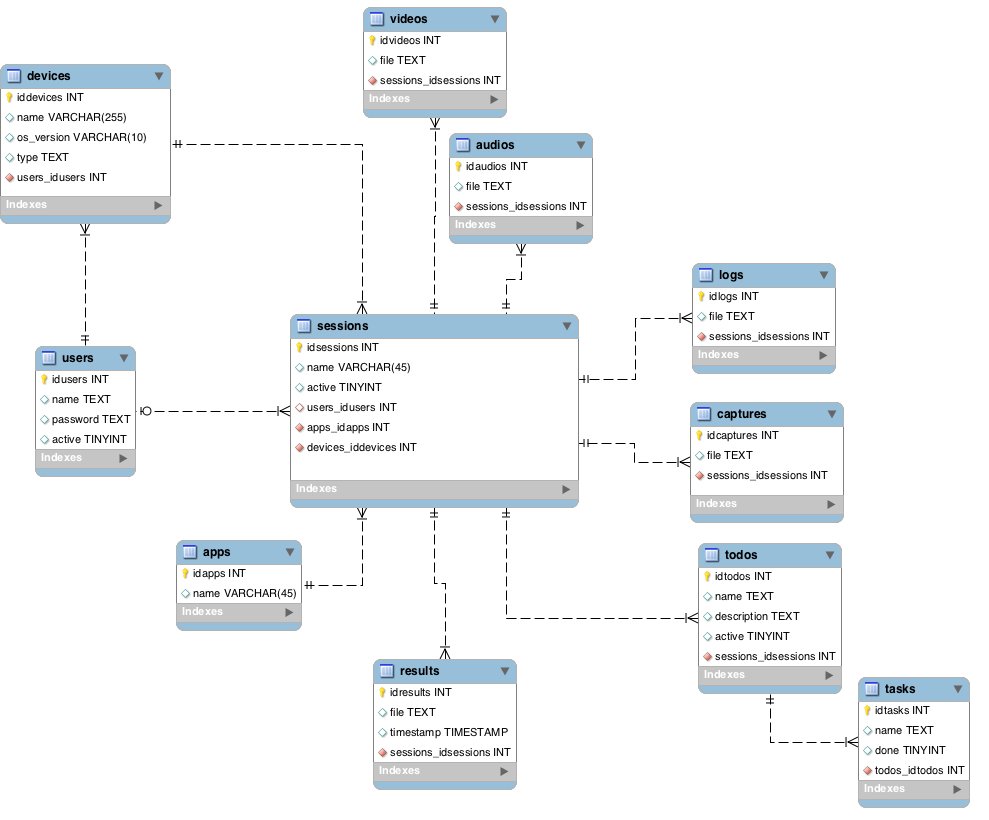
\includegraphics[width=\linewidth,keepaspectratio]{img/db_model.png}
	\caption{Datenbank Modell}
	\label{figure-db-model}
\end{figure}


\subsection{NodeJS HTTP-Server und Middleware}
Die serverseitige Logik wurde mit NodeJS und dem ExpressJS-Framework umgesetzt. Folglich wurde serverseitig Javascript eingsetzt. Javascript eigenet sich sehr für Programmierschnittstellen und HTTP-Anfragen. Nicht nur, da Javascript aus dem Web nicht mehr wegzudenken ist, sondern auch da es komplett asynchron programmiert werden kann. 

Das Express-Framework stellt die grundlegenden Funktionen eines Web-, bzw. HTTP-Servers bereit. Ein minimaler HTTP-Server ist im Listing \ref{minimal_node_http_server} zu sehen. 

\begin{lstlisting}[label=minimal_node_http_server,language=Java, caption=Minimaler Node-HTTP-Server]
/**
 * Module dependencies.
 */
var express = require('express');
var routes = require('./routes');
var http = require('http');
var path = require('path');
var app = express();

// environments config
app.set('port', process.env.PORT || 3000);
app.set('views', path.join(__dirname, 'views'));
app.set('view engine', 'ejs');
app.use(express.favicon());
app.use(express.logger('dev'));
app.use(express.json());
app.use(express.urlencoded());
app.use(express.methodOverride());
app.use(app.router);
app.use(express.static(path.join(__dirname, 'public')));

// simple test route
app.get('/ping', routes.pong);


// server take off
http.createServer(app).listen(app.get('port'), function(){
  console.log('Express server listening on port ' + app.get('port'));
});
\end{lstlisting}

\subsubsection{APIs}

\subsection{Videoproduktion}

Zur Erstellung der Zwischenergebnisse und des Endergebnisses wird die Open Source-Bibliothek \emph{libav}\footnote{} verwendet. Genauer wird die darin enthaltene Software \emph{avconv} genutzt um die Bilder und Videos zusammenzufügen. 
